\documentclass[10pt,a4paper]{article}
\usepackage[latin1]{inputenc}
\usepackage[english]{babel}

\usepackage{hyphenat}
\usepackage{fancyhdr}
\usepackage{graphicx}
\pagestyle{fancy}

\usepackage{xltxtra}
\setmainfont[Mapping=tex-text,Ligatures={Common, Historical},Numbers={OldStyle}]{OFL Sorts Mill Goudy}


% Fancy header and footer to have my name everywhere
\lhead{\textbf{Multiple scattering}}
\chead{}
\rhead{\thepage /\pageref{LastPage}}
\lfoot{}
\cfoot{}
\rfoot{}
\renewcommand{\headrulewidth}{0.4pt}
%\renewcommand{\footrulewidth}{0.4pt}

% Page formatting (A4)
\pdfpagewidth 210mm
\pdfpageheight 297mm

% Margins and other stuff
% Vertical
\setlength\voffset{4.6mm}          % 1 in is automatically added (25.4mm)
\setlength\topmargin{0mm}
\setlength\headheight{0pt}
\setlength\headsep{24pt}
%\setlength\textheight{237mm}
\setlength\textheight{225mm}
\setlength\footskip{36pt}
% Horizontal
\setlength\hoffset{0mm}
\setlength\oddsidemargin{-12.9mm}  % 1 in is automatically added (25.4mm)
\setlength\evensidemargin{-12.9mm} % 1 in is automatically added (25.4mm)
\setlength\textwidth{18.5cm}
\setlength\headwidth{18.5cm}
\setlength\marginparsep{6pt}
\setlength\marginparwidth{0mm}
% Paragraph stuff
\setlength\parindent{0mm}
\setlength\parskip{10pt}

\begin{document}
\section{Helix equation fit}
The points will lay on a helix, or (for our purposes) on a circle (we
will neglect the z axis).  The error $\varepsilon_i$ of the
measurement point $i$ will be given by:
\begin{equation}
  \label{eq:helix}
  \varepsilon_i = \frac 1 2 \rho r_i^2 - (1 + \rho d) r_i \sin(\phi_i-\phi_0) + \frac 1 2 \rho d^2 + d -y_i
\end{equation}
there $r_i$ is the layer radius, $\phi_0$ is the initial track's polar
angle in the transverse plane, $\phi_i$ is the polar angle of each
hit, $\rho$ is the curvature of the track ($\rho=1/R$, with $R$ radius
of curvature) and $d$ is the distance of closest approach of the track
to the $z$ axis.  The curvature $\rho$ is related to the transverse
momentum accoding to
\begin{equation}
  \rho (\mathrm{m}) = \frac {0.3 B} {p_T} 
\end{equation}
assuming a single-charged particle, with $B$ measured in Tesla and
$p_T$ in GeV/$c$. Assuming the CMS magnet field of 3.8~T, this becomes
\begin{equation}
  \rho (\mathrm{mm}) = \frac {1.14\times 10^3} {p_T} 
\end{equation}

We have a set of measurement points, where the only error is baically
on the $y$ position of hit $y_i = d \sin (\phi-\phi_0)$. For momenta
high enough, fitting the helix reduces to minimzing the $\chi^2$
defined as follows
\begin{equation}
  \chi^2 = \sum_{i,j} \varepsilon_j C^{-1}_{i,j} \varepsilon_i
\end{equation}
with $C_{i,j}$ the correlation between the measurement points. The
weight matrix $W$ will be:
\begin{equation}
  W_{k,l} = \sum_{i,j} \frac { \partial \varepsilon_i} {\partial \alpha_k} C^{-1}_{i,j}  \frac { \partial \varepsilon_j} {\partial \alpha_l}
\end{equation}
with $\alpha_1 = \rho$, $\alpha_2 = \phi$, $\alpha_3 = d$. The
covariance matrix $S$ is given by $S=W^{-1}$, and thus the measurement
errors are:
\begin{eqnarray}
\Delta \rho &=& \sqrt{W_{1,1}^{-1}} \nonumber \\
\Delta \phi &=& \sqrt{W_{2,2}^{-1}} \nonumber \\
\Delta d &=& \sqrt{W_{3,3}^{-1}} \nonumber
\end{eqnarray}
which can be also written as
\begin{eqnarray}
\sigma^2_\rho &=& S_{1,1} \nonumber \\
\sigma^2_\phi &=& S_{2,2} \nonumber \\
\sigma^2_d &=& S_{3,3} \nonumber \\
\sigma_{\rho, \phi} & = & S_{1,2} \nonumber \\
 & \ldots & \nonumber
\end{eqnarray}
to evidentiate the covariances. The derivatives of (\ref{eq:helix}) are:
\begin{eqnarray}
  \frac { \partial \varepsilon_i} {\partial \alpha_1} =
  \frac { \partial \varepsilon_i} {\partial \rho} &=& \frac 1 2 r_i^2 + d (d+y_i) \nonumber \\
  \frac { \partial \varepsilon_i} {\partial \alpha_2} =
  \frac { \partial \varepsilon_i} {\partial \phi} &=& - x_i (1+\rho d) \nonumber \\
  \frac { \partial \varepsilon_i} {\partial \alpha_3} =
  \frac { \partial \varepsilon_i} {\partial d} &=& 1 + \rho (d - y_i) \nonumber 
\end{eqnarray}
If we take into account that $d \ll r_i$, $d \ll 1/\rho$, $y_i \ll
1/\rho$, $r_i \simeq x_i$ we can approximate the previous set of
equations as
\begin{eqnarray}
\frac { \partial \varepsilon_i} {\partial \alpha_1} =
\frac { \partial \varepsilon_i} {\partial \rho} &=& \frac 1 2 r_i^2 \nonumber \\
\frac { \partial \varepsilon_i} {\partial \alpha_2} =
\frac { \partial \varepsilon_i} {\partial \phi} &=& - r_i  \nonumber \\
\frac { \partial \varepsilon_i} {\partial \alpha_3} =
\frac { \partial \varepsilon_i} {\partial d} &=& 1 \nonumber 
\end{eqnarray}
If we have $M$ measurement points, the partial derivatives matrix $D$
will be $M\times 3$ and defined by
\begin{equation}
  D_{i,j} = \frac { \partial \varepsilon_i} {\partial \alpha_j}
\end{equation}
and the $3\times 3$ weight matrix $W$ will be (in matrix notation)
$W=D^{T}C^{-1}D$.
\section{Error estimate}
\subsection{Track parameters}
Given the layer radii $x_n = x_1, x_2, \ldots, x_N$ with scattering
angles $\theta_1, \theta_2, \ldots, \theta_3$, then the deviation from
the ideal path $y_n$ is
\begin{equation}
  y_n=\sum_{i=1}^{n-1} \left (  x_n - x_i \right ) \theta_i
\end{equation}
The angles $\theta_i$ are distributed as a Gaussian, with r.m.s. such
that
\begin{equation}
  \left < \theta^2 \right > =
  \left ( \frac {13.6\,\mathrm{MeV}} {p} \right )^2
  \frac x {X_0}
  \left [ 1+ 0.038 \log \left ( \frac x {X_0} \right ) \right ] ^2
\end{equation}
The correlation between two deviations $y_n, y_m$ is (we will assume
without loss of generality that $m \geq n$)
\begin{equation}
  a_{n,m}\left < y_n y_m \right > =
  \left <
    \sum_{i=1}^{m-1} \left (  x_m - x_i \right ) \theta_i
    \times
    \sum_{j=1}^{n-1} \left (  x_n - x_j \right ) \theta_j
  \right >
\end{equation}
Since the angles $\theta_i$ are uncorrelated, any term containing in
$\left < \theta_i \theta_j \right >$ with $i\neq j$ will be zero, thus
\begin{eqnarray}
  a_{n,m} = \left < y_n y_m \right > & = &
  \left <
    \sum_{i=1}^{m-1} \sum_{j=1}^{n-1}
    \left (  x_m - x_i \right )
    \left (  x_n - x_j \right ) \theta_i \theta_j \delta_{i,j}
  \right > \nonumber \\
  a_{n,m} = \left < y_n y_m \right > & = &
  \sum_{i=1}^{n-1} 
  \left (  x_m - x_i \right )
  \left (  x_n - x_i \right )  \left < \theta_i^2 \right > 
\end{eqnarray}
The measurement ``error'' depends both on the scattering of the real
track with respect to the ideal case and also on the intrinsic
measurement error $\sigma_i$, which depends approximately on the strip
pitch $p_i$ according to $\sigma_i = p_i / \sqrt{12}$, or $\sigma_i^2
= p_i^2 / 12$, thus the covariance matrix $b_{n,m}$ is
\begin{equation}
  b_{n,m}= \left \{
\begin{array}{cl}
  \sum_{i=1}^{n-1} \left (  x_m - x_i \right ) \left (  x_n - x_i \right )  \left < \theta_i^2 \right > & n<m \\
  p_n^2 / 12 + \sum_{i=1}^{n-1} \left (  x_n - x_i \right )^2  \left < \theta_i^2 \right > & n=m \\
  b_{m,n}  & n>m
\end{array}
\right .
\end{equation}
Let's suppose we have $N$ hits, but in these $N$ only $M$ are
measurement points and $N-M$ are hits on inactive surfaces. In this
matrix $b_{n,m}$ is computed exactly in the same way, but the rows and
columns corresponding to the inactive hits are removed. We thus start
from a $N\times N$ square matrix of correlations $b_{n,m}$ and we end
up with a $M\times M$ measurement point covariance matrix $C_{n,m}$,
or in matrix notation $C$.


%\subsection{Extrapolation to the ECAL}
%We want to estimate the error in the extrapolation of the track to an
%external cylindrical surface, for example the inner surface of ECAL.
%
%In the transverse plane this reduces to the interception of two
%circles: the given cylinder section of radius $L$ and the track
%trajectory with radius $R=1/\rho$. Given that typically $R \gg d$ and
%$L \gg d$ we will neglect $d$ and consider the particle trajectory to
%be starting from the origin of the ${x, y}$ plane (see
%Figure~\ref{fig:angle} below).
%\begin{figure}[h]
%\begin{center}
%\includegraphics[height=0.5\textwidth,angle=-90]{angle.pdf}
%\caption{Target cylinder surface and particle trajectory in the ${x, y}$ plane}
%\label{fig:angle}
%\end{center}
%\end{figure}
%
%To extrapolate the position on the target barrel the important
%parameter is $\varphi$:
%\begin{equation}
%\varphi = \phi + \beta
%\end{equation}
%where $\phi$ is the trajectory angle at the origin already esitmated
%(plus a constant which is not influent in the error estimation) and
%$\beta$ is shown in Figure~\ref{fig:angle}.
%
%From the figure one can easily get the relation
%\begin{eqnarray}
%  R \, \cos(\beta) & =& \frac L 2 \\
%  \beta & = & \arccos \left ( \frac {L \rho} 2 \right )
%\end{eqnarray}
%where the relation $R = 1/ \rho$ was used.
%
%The error on $\varphi$ can be estimated through
%\begin{equation}
%\sigma^2_{\varphi} = \left ( \frac {\partial \varphi} {\partial \rho} \right )^2 \sigma^2_{\rho}
%+ \left ( \frac {\partial \varphi} {\partial \phi} \right )^2 \sigma^2_{\phi}
%+ 2 \left ( \frac {\partial \varphi} {\partial \rho} \right ) \left ( \frac {\partial \varphi} {\partial \phi} \right ) \sigma_{\phi \rho}
%\end{equation}
%given that
%\begin{equation}
%\frac {\partial \varphi} {\partial \phi} = 1
%\end{equation}
%and
%\begin{equation}
% \frac {\partial \varphi} {\partial \rho} = 
% \frac {\partial \beta} {\partial \rho} = 
%- \frac {L} {\sqrt{4 - {L^2 \rho^2} }}
%\end{equation}
%the error on $\varphi$ can be written as
%\begin{equation}
%\sigma^2_{\varphi} = \left ( \frac {L^2 } {4 - L^2 \rho^2 } \right )  \sigma^2_{\rho}
%+ \sigma^2_{\phi}
%-  \left ( \frac {2\,L} {\sqrt{4- {L^2 \rho^2} }} \right ) \sigma_{\phi \rho}
%\end{equation}
%the linear error in the $r-\varphi$ plane of the extrapolation $\Delta s$ will be finally
%\begin{equation}
%\Delta s = L \sqrt{\sigma^2_{\varphi}}
%\end{equation}
%

\section{Impact parameter quality}
We assume that the primary vertex is known with a much better
precision than the impact paramteter, so we place our reference system
with the origin in the primary vertex.

\begin{figure}[h]
\begin{center}
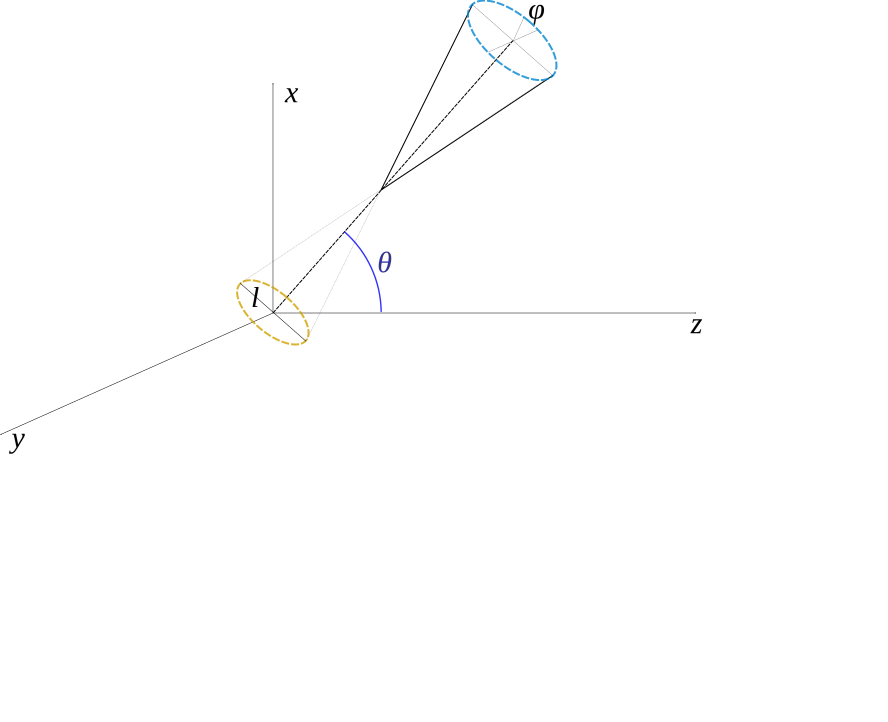
\includegraphics[height=0.5\textwidth]{impact_parameter.pdf}
\caption{Impact parameter}
\label{fig:impact}
\end{center}
\end{figure}

For symmetry reasons we can assume that the meson we want to identify
is created in the $\{x,z\}$ plane. The angle between the direction of
flight and the $z$ axis is $\vartheta$.

The decay happens after a distance $f$, and the angle between the
tracked decay product and the original meson is $\alpha$.

The projection of the track on the plane containing the origin and
perpendicular to the meson line of flight will be on a circle of
radius $l=f\,\sin(\alpha)$. It can be noted that $f=\gamma\,c\,\tau$
and $\alpha \simeq 1/\gamma$, thus
\begin{equation}
l \simeq c \, \tau
\end{equation}

Said plane will have axes $\vec{e_{x'}}$ and $\vec{e_y}$, with
\begin{equation}
  \vec{e_{x'}} = \vec{e_x}\,\cos(\vartheta) - \vec{e_z}\,\sin(\vartheta)
\end{equation}

If we call $\phi$ the angle running on this circle, the projection point has equation
\begin{equation}
\left \{
\begin{array}{rcl}
x' & = & l\,\sin(\phi) \\
y  & = & l\,\cos(\phi) \\
z '& = & 0
\end{array}
\right .
\end{equation}
that is
\begin{equation}
\left \{
\begin{array}{rcl}
x & = &  l\,\sin(\phi)\,\cos(\vartheta) \\
y & = &  l\,\cos(\phi) \\
z & = & -l\,\sin(\phi)\,\sin(\vartheta)
\end{array}
\right .
\end{equation}

Assuming we can measure the transverse impact parameter with
resolution $\sigma_{d0}$ and the longitudinal impact parameter with
resolution $\sigma_{z0}$, then we want to combine these two
measurements into one parameter $t$. In the $\{d_0, z_0\}$ plane the
origin is $\frac{d_0}{\sigma_{d0}}$ standard deviations away along one
axis and $\frac{z_0}{\sigma_{z0}}$ standard deviations away along the
other, so a reasonable discriminant is
\begin{equation}
t^2 = \left ( \frac {r} {\sigma_{d0}} \right )^2 + 
              \left ( \frac {z} {\sigma_{z0}} \right )^2
\end{equation}
with $r^2=x^2+y^2$ which leads to:
\begin{equation}
t^2 = \frac {l^2\,\cos^2(\vartheta)\,\sin^2(\phi) + l^2\,\cos^2(\phi)} {\sigma_{d0}^2} + 
    \frac {l^2\,\sin^2(\vartheta)\,\sin^2(\phi)} {\sigma_{z0}^2}
\end{equation}
Averaging on $\phi$ gives:
\begin{equation}
  t^2 = \frac {l^2} {2} \left [ \frac {\cos^2(\vartheta) + 1 } {\sigma_{d0}^2} + 
        \frac {\sin^2(\vartheta)} {\sigma_{z0}^2} \right ]
\end{equation}
The significance $t$ can thus be interpreted as the proper decay
length $l$ divided by its measurement error:
\begin{equation}
\frac {l} {\sigma_l} = l \, \sqrt{ \frac 1 2 \left [ \frac {\cos^2(\vartheta) + 1 } {\sigma_{d0}^2} + 
                                   \frac {\sin^2(\vartheta)} {\sigma_{z0}^2} \right ] }
\end{equation}
and 
\begin{equation}
\sigma_l = \frac 1 { \sqrt{ \frac 1 2 \left [ \frac {\cos^2(\vartheta) + 1 } {\sigma_{d0}^2} + 
                                   \frac {\sin^2(\vartheta)} {\sigma_{z0}^2} \right ] } }
\end{equation}
and finally:
\begin{equation}
\sigma_l = \sqrt{ \frac 2 {  \frac {\cos^2(\vartheta) + 1 } {\sigma_{d0}^2} + 
                                   \frac {\sin^2(\vartheta)} {\sigma_{z0}^2} } }
\end{equation}
considering that $\gamma \gg 1$, then $\alpha \ll 1$ and thus the track angle $\theta \simeq \vartheta$.

\begin{equation}
\sigma_{c\tau} = \sqrt{ \frac 2 {  \frac {\cos^2(\theta) + 1 } {\sigma_{d0}^2} + 
                                   \frac {\sin^2(\theta)} {\sigma_{z0}^2} } }
\end{equation}

When looking at possible optimizations, one possible measurement is
the relative increase of $\sigma_{c\tau}$ for an increase of $\sigma_{d0}$ and $\sigma_{z0}$
\begin{equation}
F(\theta, \sigma_{d0}, \sigma_{z0}) =
\frac
  {\frac {\partial \sigma_{c\tau}} {\partial \sigma_{d0}} }
  {\frac {\partial \sigma_{c\tau}} {\partial \sigma_{z0}} } = 
\frac
  {(\cos^2(\theta) + 1)\, \sigma^3_{z0}}
  {\sin^2(\theta) \, \sigma^3_{d0}}
\end{equation}
This function $F$ could tell the relative gain of increasing
$\sigma_{d0}$ or $\sigma_{z0}$. One easy way of representing it is
$\beta = \arctan (F(\theta, \sigma_{d0}, \sigma_{z0}) )$. When $\beta
\simeq 0$ the resolution is dominated by $\sigma_{z0}$ and when $\beta
\simeq \pi/2$ the resolution is dominated by $\sigma_{d0}$.

Another parameter for optimization comes from the observation that, to
the first order, the resolution is proportional to the pixel size and
that for a fixed channel count, one can double the resolution on one
axis by halfening it on the other. In these terms it makes sense to
express the resolutions as a function of their product
$k=\sigma_{z0}\times\sigma_{d0}$ (which can be taken as a constraint)
and their ratio $x=\sigma_{z0}/\sigma_{d0}$, which can be
considered our optimization free variable (higher $x$ means longer pixels). We want to maximize
$B=1/\sigma^2_l$, that is
\begin{equation}
  B = \frac 1 2 \left [ \frac {\cos^2(\theta)+1} {k/x} + \frac {\sin^2(\theta)} {k\,x} \right ]
\end{equation}
\begin{equation}
 \frac { \partial B } {\partial x} = \frac { \cos^2(\theta) + 1 + \frac 1 x \sin^2(\theta) } {2\,k}
\end{equation}
As usual we can express this as an angle $\Omega=\arctan(\partial B /
\partial x)$. For $\Omega = \pi/2$ it is better to have longer pixels
and for $\Omega = -\pi/2$ it is better to have shorter (and wider)
pixels. The optimal compromise is reached for $\Omega \simeq 0$.


\label{LastPage}
\end{document}
